\let\negmedspace\undefined
\let\negthickspace\undefined
\documentclass[journal,onecolumn]{IEEEtran}

\usepackage[a5paper, margin=10mm]{geometry} % Safe with onecolumn
\usepackage{lmodern} % Better fonts (optional but recommended)
\usepackage{tfrupee} % Rupee symbol package

% Header fix
\setlength{\headheight}{12pt} % Safe value
\setlength{\headsep}{0pt}     % Reduce gap

\usepackage{gvv-book}
\usepackage{gvv}
\usepackage{cite}
\usepackage{amsmath,amssymb,amsfonts,amsthm}
\usepackage{algorithmic}
\usepackage{graphicx}
\usepackage{textcomp}
\usepackage{xcolor}
\usepackage{txfonts}
\usepackage{listings}
\usepackage{enumitem}
\usepackage{mathtools}
\usepackage{gensymb}
\usepackage{comment}
\usepackage[breaklinks=true]{hyperref}
\usepackage{tkz-euclide} 
\usepackage{listings}
% \usepackage{gvv}                                        
\def\inputGnumericTable{}                                 
\usepackage[latin1]{inputenc}                                
\usepackage{color}                                            
\usepackage{array}                                            
\usepackage{longtable}                                       
\usepackage{calc}                                             
\usepackage{multirow}                                         
\usepackage{hhline}                                           
\usepackage{ifthen}                                           
\usepackage{lscape}

\usepackage{amsmath,amssymb}
\usepackage{booktabs}
\usepackage{tikz}
\usetikzlibrary{arrows.meta,angles,quotes}

\begin{document}

\bibliographystyle{IEEEtran}
\vspace{3cm}

\title{4.13.19}
\author{EE25BTECH11014 - Bhoomika Lokesh}
% \maketitle
% \newpage
% \bigskip
{\let\newpage\relax\maketitle}

\renewcommand{\thefigure}{\theenumi}
\renewcommand{\thetable}{\theenumi}
\setlength{\intextsep}{10pt} % Space between text and floats

% Remove this line so equations use default numbering (1, 2, 3,...)
% \numberwithin{equation}{enumi}
\numberwithin{figure}{enumi}
\renewcommand{\thetable}{\theenumi}


\textbf{Question:}If the line $2x+y=k$ passes through the point which divides the line segment joining the points $\brak{1,1}$ and $\brak{2,4}$ in the ratio 3:2, then $k$ equals
\begin{multicols}{4}
\begin{enumerate}
    \item $\frac{29}{5}$
    \item $5$
    \item $6$
    \item $\frac{11}{5}$
\end{enumerate}
\end{multicols}

\textbf{Solution:}\\
Let the point $\vec{C}$ divide the line segment joining $\vec{A}$ and $\vec{B}$ in the ratio 3:2\\
where\begin{align}
    \vec{A}=\myvec{1\\1}\\
    \vec{B}=\myvec{2\\4}
\end{align}
By section formula,
\begin{align}
   \vec{C}=\frac{\lambda\vec{B}+\vec{A}} {\brak{\lambda +1}}.\\  
    Here \brak{\lambda=\frac{3}{2}}
\end{align}

The equation of the line can be represented as:
\begin{align}
    \vec{n^T}\vec{x}=c_1\\
 where  \ \vec{n^T}=\myvec{2&1} \ and \ c_1=k.
\end{align}
As $\vec{C}$ lies on the above line,
\begin{align}
  \vec{n^T}\vec{C}=c_1\\
 \myvec{2&1}\frac{\lambda\vec{B}+\vec{A}} {\brak{\lambda +1}}=k\\
 \frac{1}{5}\myvec{2&1}\brak{3\vec{B}+2\vec{A}}=k\\
 \frac{1}{5}\myvec{2&1}\brak{\myvec{6\\12}+\myvec{2\\2}}=k\\
 \frac{1}{5}\myvec{2&1}\myvec{8\\14}=k\\
 k=\frac{16}{5}+\frac{14}{5}=6.
\end{align}

\begin{figure}[H]
\begin{center}
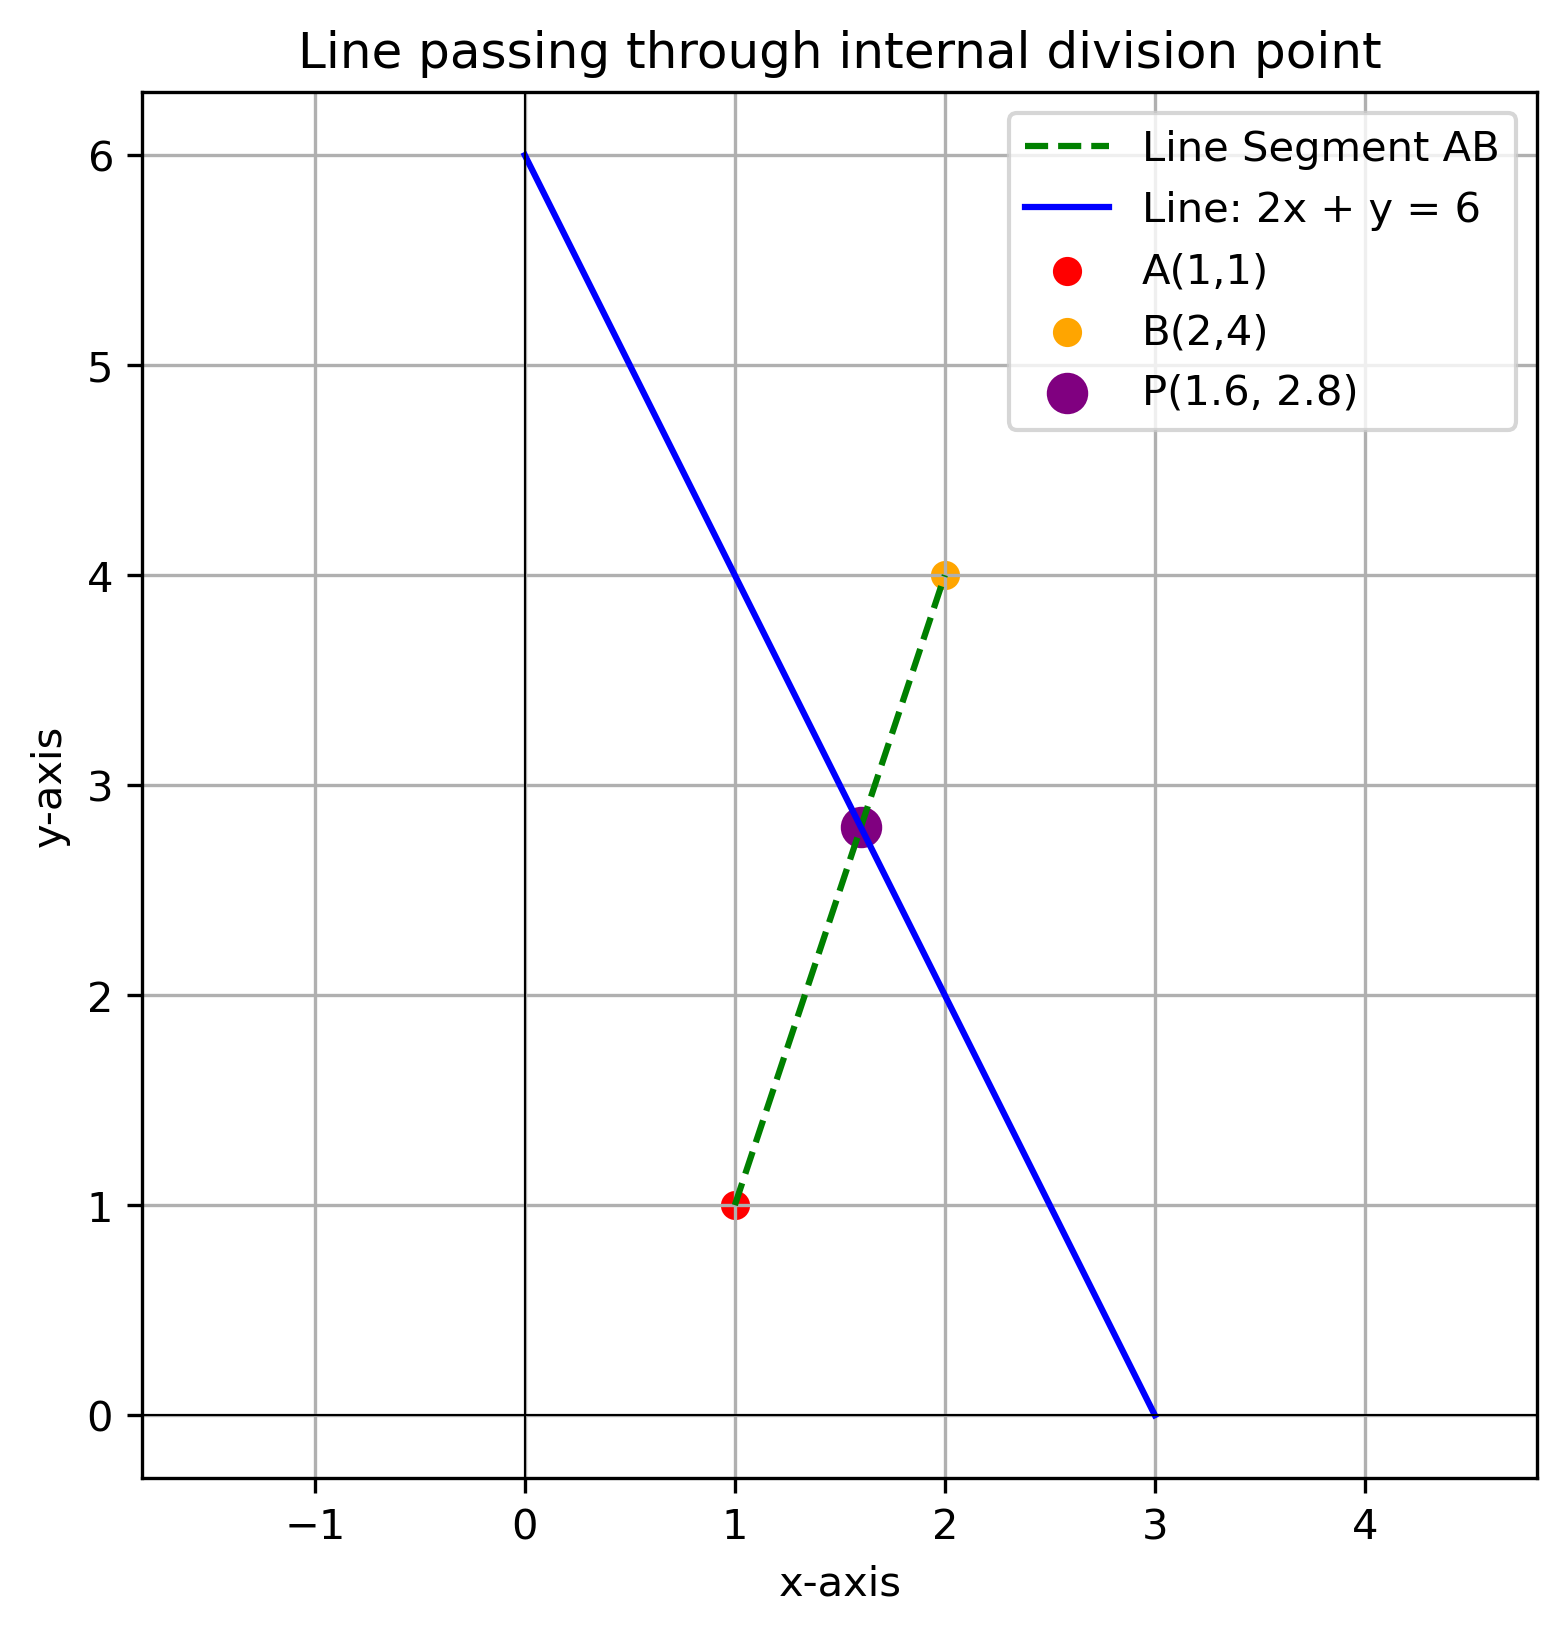
\includegraphics[width=0.7\columnwidth]{Figs/findk.png}
\end{center}
\caption{Graph}
\label{fig:fig.py}
\end{figure}

\end{document}